\documentclass[11pt]{article}
%Importing custom commands
\usepackage{latex_goon/latex_goon}
\title{Decoder-Only Transformers}
\author{Garrett Goon}
\begin{document}
%
%\maketitle

\vspace{1truecm}
%
%
\renewcommand{\thefootnote}{\fnsymbol{footnote}}
\begin{center}
{\huge \bf{Decoder-Only Transformers}}
\end{center}


\begin{abstract}

Notes on various aspects of Decoder-Only Transformers.

\end{abstract}

\tableofcontents


\renewcommand*{\thefootnote}{\arabic{footnote}}
\setcounter{footnote}{0}

\part{Architecture}

\section{Decoder-Only Fundamentals \label{sec_decoder_only} }

The Transformers architecture \cite{vaswani2017attention}, which dominates Natural Language
Processing (NLP) as of July 2023, is a relatively simple architecture. There are various flavors and
variants of Tranformers, but focus here on the decoder-only versions which underlie the
GPT models \cite{gpt2radford2019language, gpt3brown2020language, gpt4openai2023}.

The full decoder-only architecture can be seen in Fig.~\ref{fig_transformers_architecture}. The
parameters which define the network can be found in App.~\ref{app_conventions}.
\begin{figure}[ht]
    \centering
    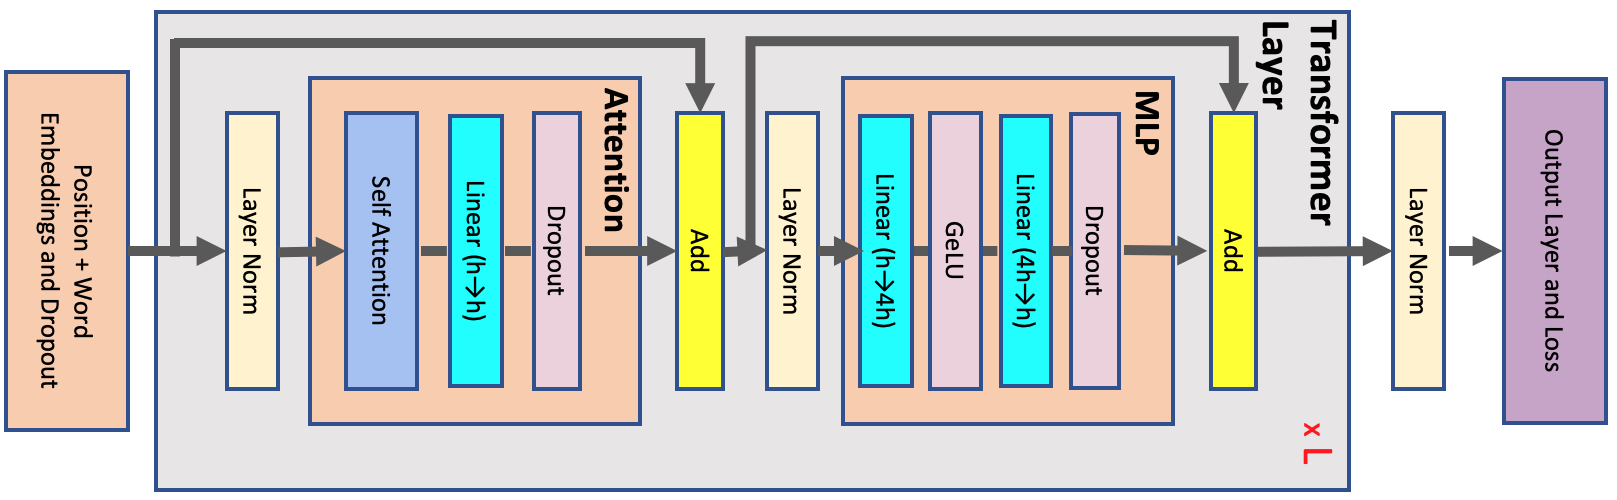
\includegraphics[scale=0.28]{figures/transformer-general.jpg}
    \caption{The full transformers architecture. Diagram taken from \cite{korthikanti2022reducing} }
    \label{fig_transformers_architecture}
\end{figure}


At a high level, decoder-only transformers take in a series of word-like objects, called tokens, and are trained
to predict the next token in the sequence. An outline of the mechanics:
\begin{enumerate}
    \item Raw text is \textbf{tokenized} and turned into a series of integers\footnote{There are
        about \href{https://github.com/ray-project/llm-numbers}{1.3 tokens per word}, on average.} whose values lie in \pyinline{range(V)}, with $ V $ the vocabulary
        size.
    \item The tokenized text is chunked and turned into \pyinline{(B, S)}-shaped (batch size and
        sequence length, respectively) integer tensors, $ x _{ bs } $.
    \item The \textbf{embedding layer} converts the integer tensors into continuous representations of shape
        \pyinline{(B, S, D)}, $ z _{ bsd } $, with $ D $ the size of the hidden dimension.
        \textbf{Positional encodings} have also been added to the tensor at this stage to help the
        architecture understand the relative ordering of the text.
    \item The $ z _{ bsd } $ tensors pass through a series of transformer blocks, each of which has
        two primary components:
        \begin{enumerate}
        \item In the \textbf{attention} sub-block, components of $ z _{ bsd } $ at different
            positions ($ s $-values) interact with each other, resulting in another \pyinline{(B, S, D)}-shaped
            tensor, $  z' _{ bsd } $.
        \item In the \textbf{MLP} block, each position in  $ z' _{ bsd } $ is processed
            independently and in parallel by a two-layer feed-forward network, resulting once more
            in a \pyinline{(B, S, D)}-shaped tensor.
        \end{enumerate}
        Importantly, there are \textbf{residual connections} around each of these\footnote{This
        gives rise to the concept of the \textbf{residual stream} which each transformer block reads
        from and writes back to repeatedly.} (the arrows in Fig.~\ref{fig_transformers_architecture}).
    \item Finally, we convert the \pyinline{(B, S, D)}-shaped
        tensors to \pyinline{(B, S, V)}-shaped ones, $ y _{ bsv } $. This is the role of
        the \textbf{language model head} (which is often just the embedding layer used in an inverse
        manner.)
    \item  The $ y _{ bsv } $ predict what the next token will be, i.e. $ x _{ bs+1 } $, having seen the \textbf{context}
        of the first $ s $ tokens in the sequence.
\end{enumerate}


Each batch (the $ b $-index) is processed independently. We omitted \pyinline{LayerNorm} and
\pyinline{Dropout} layers above, as well as the causal mask; these will be covered below as we step
through the architecture in more detail.


We break down the various components below in detail.

\subsection{Embedding Layer and Positional Encodings \label{subsubsec_embedding_and_pe} }

The \textbf{embedding} layer is just a simple look up table: each of the \pyinline{range(V)} indices
in the vocabulary is mapped to a $ D $-dimensional vector via a large \pyinline{(V, D)}-shaped
table/matrix. This layer maps $ x _{ bs } \longrightarrow z _{ bsd } $. In \pyinline{torch}, this is
an \pyinline{nn.Embedding(V, D)} instance.

To each item in a batch, we add identical \textbf{positional encodings} to the vectors above with
the goal of adding fixed, position-dependent correlations in the sequence dimension which will
hopefully make it easier for the architecture to pick up on the relative positions of the inputs
\footnote{Positional encodings and the causal mask are the only components in the transformers
architecture which carry weights with a dimension of size $ S $; i.e. they are the only parts that
have explicit sequence-length dependence. A related though experiment: you can convince yourself
that if the inputs $ z_{ bsd } $
were just random noise, the transformers architecture would not be able to predict
the $ s $-index of each such input in the absence of positional encodings. } This layer maps $ z _{
bsd} \leftarrow z _{ bsd } + p _{ sd } $, with $ p _{ sd } $ the positional encoding tensor.

The above components require $ (V+S)D \approx VD $ parameters per layer.



\subsection{Layer Norm \label{subsubsec_layer_norm} }

The original transformers paper \cite{vaswani2017attention} put \pyinline{LayerNorm} instances after
the \textbf{attention} and \textbf{MLP} blocks, but now it is common \cite{xiong2020layer} to put
them before these blocks\footnote{Which makes intuitive sense for the purposes of stabilizing the
matrix multiplications in the blocks}.

The \pyinline{LayerNorm} operations acts over the sequence dimension. Spelling it out, given the
input tensor $ z _{ bsd } $ whose mean and variance over the $ s $-index are $ \mu _{ bd } $ and $
\sigma _{ bd } $, respectively, the \pyinline{LayerNorm} output is
\begin{align}
  z _{ bsd } &\leftarrow \left ( \frac{ z _{ bsd } - \mu _{ bd } }{ \sigma _{ bd } } \right )\times \gamma _{ d }
  + \beta _{ d } \equiv \LN _{ s } z _{ bsd}
\end{align}
where $ \gamma _{ d }, \beta  _{ d } $ are the trainable scale and bias parameters. In
\pyinline{torch}, this is a \pyinline{nn.LayerNorm(D)} instance.

Since there are two \pyinline{LayerNorm} instances in each transformer block, these components require
$ 2D $ parameters per layer.


\subsection{Causal Attention \label{subsubsec_attn_layer} }

The \textbf{causal attention} layer is the most complex layer. It features $ A $  triplets\footnote{$ A $
must divide the hidden dimension $ D $ evenly.} of weight matrices\footnote{There are also bias
terms, but we will often neglect to write them explicitly or account for their (negligible)
parameter count.}  $ Q ^{ a } _{ d f }, K ^{ a } _{ df }, V ^{ a } _{ df }  $
where $ a \in \left \{ 0, \ldots, H-1 \right \} $ and $ f \in \left \{ 0, \ldots, D/A \right \} $.
From these, we form three different vectors:
\begin{align}
  q ^{ a }_{ bsf } &= z _{ bsd } Q ^{ a }_{ df } \ , \quad
  k ^{ a }_{ bsf } = z _{ bsd } K ^{ a }_{ df }  \ , \quad
  v ^{ a }_{ bsf } = z _{ bsd } V ^{ a }_{ df }
\end{align}
These are the \textbf{query, key, and value} tensors, respectively \footnote{There are of course
many variants of the architecture and one variant which is popular in Summer 2023 is multi-query
attention \cite{shazeer2019fast} in which all heads share \textit{the same} key and value vectors
and only the query changes across heads, as this greatly reduces inference costs.}.

Using the above tensors, we will then build up an \textbf{attention map}  $ w ^{ a }_{ bss' } $
which corresponds to how much attention the token at position $ s $ pays to the token at
position $ s' $.  Because we have the goal of predicting the
next token in the sequence, we need these weights to be causal: the final prediction $ y _{ bsv } $
should only have access to information propagated from positions $ x _{ bs'v } $ with $ s' \le s $.
This corresponds to the condition that $ w ^{ a }_{ bss' } = 0  $ if  $ s' > s  $.

 These weights come from \pyinline{Softmax}-ed attention scores, which are just a normalized
 dot-product over the hidden dimension:
\begin{align}
    w ^{ a }_{ bss'd } &=\Sm _{ s' } \left (m _{ s s' }+\ q ^{ a }_{ bsf }k ^{ a }_{ bs'f } / \sqrt{D/A} \right
        )\ ,  \quad {\rm s.t.} \quad \sum_{s'}w ^{ a }_{ bdss' } =1
\end{align}
The tensor $ m _{  s s' } $ is the causal mask which zeroes out the relevant attention map
components above
\begin{align}
    m _{ s s' } &= \begin{cases}
            0 & s \le s' \nn
            -\infty &= s > s'
        \end{cases}\ ,
\end{align}
forcing $ w ^{ a  } _{ bss'd } =0$ for $ s> s' $. In other words, the causal mask ensures that a
given tensor, say $ z _{ bsd } $, only has dependence on other tensors whose sequence index, say $
s' $, obeys $ s' \le s $.  This is crucial for inference-time optimizations, in particular the use
of the \textbf{kv-cache} in which key-value pairs do not need to be re-computed.

The $ \sqrt{D/A} $ normalization is motivated by demanding
that the variance of the \pyinline{Softmax} argument be 1 at initialization, assuming that other
components have been configured so that that the query and key components are i.i.d. from a Gaussian
normal distribution \footnote{However, in \cite{yang2022tensor} it is instead argued that no square
root should be taken in order to maximize the speed of learning via SGD.}.

The weights above are then passed through a dropout layer and used to re-weigh the \textbf{value} vectors and form the tensors
\begin{align}
  t ^{ a }_{ bsf }&=\Dr  \left (w ^{ a }_{ bdss' } \right ) v ^{ a }_{ bs'f }
  \label{eq_reweighted_values}
\end{align}
and these $ A $ different \pyinline{(B, S, D/A)}-shaped tensors
are then concatenated along the $ f $-direction to re-form a \pyinline{(B, S, D)}-shaped
tensor\footnote{It is hard to come up with good index-notation for concatenation.}
\begin{align}
    u _{ bsd } &= {\rm Concat}^{ a }_{ fd } \left ( t ^{ a }_{ bsf }\right )\ .
\end{align}
Finally, another weight matrix $ O _{d' d } $ and dropout layer transform the output once again to get the final
output
\begin{align}
  z _{ bsd } &= \Dr \left (u  _{ bsd' } O _{ d'd }\right )\ .
\end{align}

For completeness, the entire operation in condensed notation with indices left implicit is:
\begin{align}
    z  &\leftarrow \Dr \left ({\rm Concat} \ \left ( \Dr \left (\Sm  \left ( \frac{ \left ( z \cdot Q ^{ a } \right )\cdot \left ( z \cdot K ^{ a } \right )}{ \sqrt{D/A} }
            \right)\right )\cdot z \cdot V ^{ a } \right ) \cdot O \right ) \label{eq_causal_attn}
\end{align}
where all of the dot-products are over feature dimensions (those of size $ D $ or $ D/A $).

Below is pedagogical\footnote{The
code is written for clarity, not speed. An example optimization missing here: there is no need to
form separate $ Q ^{ a },K ^{ a },V ^{ a} $ \pyinline{Linear} layers, one large layer which is later
chunked is more efficient} sample code for such a  \pyinline{CausalAttention} layer\footnote{When
using sequence-parallelism, it will be more natural to separate out the final \pyinline{Dropout} layer
and combine it with the subsequent \pyinline{LayerNorm}, as they are sharded together; see
Sec.~\ref{subsec_seq_parallelism}.}:\pyfile[firstline=10,lastline=58]{python/causal_attention.py}

The parameter count is dominated by the weight matrices which carry $ 4 D ^{ 2 } $ total parameters per layer.


\subsection{MLP \label{subsubsec_mlp} }

The feed-forward network is straightforward and corresponds to
\begin{align}
  z _{ bsd } &\leftarrow \Dr \left (\phi \left ( z _{ bsd' }W ^{ 0 }_{ d'e } \right ) W ^{ 1 } _{ ed
      } \right ) \label{eq_mlp}
\end{align}
where $ W ^{ 0 } $ and $ W ^{ 1 } $ are \pyinline{(D, ED)}- and \pyinline{(ED, D)}-shaped matrices,
respectively (see App.~\ref{app_conventions} for notation) and $ \phi $ is a
non-linearity\footnote{The \pyinline{GeLU}
\href{https://pytorch.org/docs/stable/generated/torch.nn.GELU.html}{non-linearity} is common.}.
In code, where we again separate out the last \pyinline{Dropout} layer as we did in in
Sec.~\ref{subsubsec_attn_layer}.  \pyfile[firstline=8, lastline=23]{python/mlp.py}

This bock requires $ 2 E D ^{ 2 } $ parameters per layer, only counting the contribution from
weights.


\subsection{Language Model Head \label{subsubsec_language_model_head} }


The layer which converts the \pyinline{(B, S, D)}-shaped outputs, $ z _{ bsd } $, to \pyinline{(B, S, V)}-shaped
predictions over the vocabulary, $  y _{ bsv } $, is the \textbf{Language Model Head}. It
is a linear layer, whose weights are usually tied to be exactly those of the initial embedding
layer of Sec.~\ref{subsubsec_embedding_and_pe}.


\subsection{All Together}
It is then relatively straightforward to tie everything together.  In code, we can first create a
transformer block like
\pyfile[firstline=10, lastline=38]{python/transformer_block.py}
which corresponds to the schematic function
\begin{align}
  z &\leftarrow  z + \texttt{MLP}\left ( \LN \left ( z + \texttt{CausalAttention}\left ( \LN \left (
  z\right ) \right )  \right ) \right )\ ,
\end{align}
indices suppressed.

And then the entire architecture: \pyfile[firstline=9, lastline=50]{python/decoder_only.py}


\subsection{The Loss Function}

The last necessary component is the loss function. The training loop data is canonically the
\pyinline{(B, K)}-shaped\footnote{\pyinline{K} is the block size, the maximum sequence-length for
the model. See App.~\ref{app_conventions}.}  token inputs ($ x _{ bs } $) along with their shifted-by-one relatives $ y
_{ bs }$ where \pyinline{x[:, s + 1] == y[:, s]}.  The \pyinline{(B, K, V)}-shaped
outputs ($ z _{ bsv } $)  of the \pyinline{DecoderOnly} network are treated as the logits which
predict the value of the next token, given the present context:
\begin{align}
    p(x _{ b (s+1) }=v| x _{ b s }, x _{ b (s-1) }, \ldots, x _{ b 0 }) &= \Sm _{ v }\ z _{ bsv
    }\label{eq_transformer_conditional_prob}
\end{align}
and so the model is trained using the usual cross-entropy/maximum-likelihood loss
\begin{align}
  \Lcal(x, z) &= \frac{ 1 }{ BK }\sum _{ b,s }\ln p(x _{ b (s+1) }=| x _{ b s }, x _{ b (s-1) },
  \ldots, x _{ b 0 })\nn
  &= \frac{ 1 }{ BK }\sum _{ b,s }\Sm _{ v }\ z _{ bsv}\big| _{ v=y _{ bs } } \ .
\end{align}
Note that the losses for all possible context lengths are included in the sum.

In \pyinline{torch}
code, the loss computation might look like the following (using fake data):
\pyfile[firstline=10, lastline=23]{python/loss.py}

\part{Training}

\section{Memory \label{sec_memory_training}}

In this section we summarize the train-time memory costs of Transformers under various training
strategies\footnote{A nice related blog post is \href{https://blog.eleuther.ai/transformer-math/}{here}. \label{foot_eleuther_math_101} }.

The memory cost is much more than simply the cost of the model
parameters. Significant factors include:
\begin{itemize}
\item Optimizer states, like those of \pyinline{Adam}
\item Mixed precision training costs, due to keeping multiple model copies.
\item Gradients
\item Activation memory\footnote{Activations refers to any intermediate value which needs to be
    cached in order to compute backpropagation. We will be conservative and assume that the inputs
of all operations need to be stored, though in practice gradient checkpointing and recomputation
allow one to trade caching for redundant compute. In particular, flash attention
\cite{dao2022flashattention} makes use of this strategy.} , needed for backpropagation.
\end{itemize}
Because the activation counting is a little more involved, it is in its own section.


\begin{nicebox}{Essentials}
Memory costs count the elements of all tensors in some fashion, both from model parameters and
intermediate representations. The gradient and optimizer state costs scale with the former quantity:
$ \Ocal \left ( N _{ {\rm params}  } \right ) \sim \Ocal \left ( L D ^{ 2 } \right )$, only counting
the dominant contributions from weight matrices. Activation memory scales with the latter,
which for a \pyinline{(B, S, D)}-shaped input gives $ \Ocal \left ( BDLS  \right ) $ contributions
from tensors which preserve the input shape, as well as $ \Ocal \left( BHLS ^{ 2 } \right)  $
factors from attention matrices.
\end{nicebox}


\subsection{No Sharding}

Start with the simplest case where there is no sharding of the model states. Handling the different
parallelism strategies later will be relatively straightforward, as it involves inserting just a few
factors here and there.

\subsubsection{Parameters, Gradients, Optimizer States, and Mixed Precision
\label{sec_params_grads_optim_mem}}


Memory from the bare parameter cost, gradients, and optimizer states are fixed costs independent of
batch size and sequence-length (unlike activation memory), so we discuss them all together here. The
parameter and optimizer costs are also sensitive to whether or not mixed-precision is used, hence we
also address that topic, briefly.  We will assume the use of \pyinline{Adam}\footnote{Which stores
    \href{https://pytorch.org/docs/stable/generated/torch.optim.Adam.html}{two different running
averages} per-model parameter.} throughout, for simplicity and concreteness. It will sometimes be
useful below to let $ p $ to denote the precision in bytes that any given element is stored in, so
\pyinline{torch.float32} corresponds to $ p=4 $, for instance. Ultimately, we primarily consider
vanilla training in $ p=4 $ precision and \pyinline{torch.float32}/\pyinline{torch.float16} ($ p=4
$/ $ p=2 $)  mixed-precision, other, increasingly popular variants to exist, so we keep the
precision variable where we can.


Without mixed precision, the total cost of the
\pyinline{torch.float32} ($ p=4 $ bytes) model and optimizer states in bytes is then
\begin{align}
    M ^{ \rm model} &= 4 N _{ \rm params } \ , \quad M^{ \rm  optim } = 8 N _{ \rm params }
    \quad ({\rm no \ mixed \ precision, } p=4)
    \label{eq_optimizer_states_mem_no_mp}
\end{align}
here, from the previous section, the pure parameter-count of the decoder-only Transformers
architecture is
\begin{align}
    N _{ \rm params } &\approx  (4 + 2E) L D ^{ 2 } \times \left ( 1 + \Ocal \left( \frac{ V }{ DL }
    \right) + \Ocal \left( \frac{ 1 }{ D } \right)  \right ) \ . \label{eq_approx_params_no_sharding}
\end{align}
where the first term comes from the \pyinline{TransformerBlock} weight matrices, the first omitted
subleading correction term is the embedding matrix, and the last comes from biases,
\pyinline{LayerNorm} instances, and other negligible factors. \footnote{For the usual $ E=4 $ case,
    the \pyinline{MLP} layers are twice as costly as the \pyinline{CausalAttention} layers.} The
    optimizer states cost double the model itself.


The situation is more complicated when mixed-precision is used \cite{micikevicius2018mixed}.
The pertinent components of mixed-precision:
\begin{itemize}
\item A half-precision ($ p=2 $ bytes) copy of the model is used to perform the forwards and
    backwards passes
\item A second, "master copy" of the model is also kept with weights in full $ p=4 $ precision
\item The internal \pyinline{Adam} states are kept in full-precision
\end{itemize}
Confusingly, the master copy weights are usually accounted for as part of the optimizer state, in
which case the above is altered to
\begin{align}
    M ^{ \rm model} &= 2 N _{ \rm params } \ , \quad M^{ \rm  optim } = 12 N _{ \rm params }
    \quad ({\rm mixed \ precision}) .
    \label{eq_optimizer_states_mem_mp}
\end{align}
The optimizer state is now six times the cost of the actual model used to process data and the costs
of \eqref{eq_optimizer_states_mem_mp} are more than those of \eqref{eq_optimizer_states_mem_no_mp}.
However, as we will see, the reduced cost of activation memory can offset these increased costs, and
we get the added benefit of increased speed due to specialized hardware. The above also demonstrates
why training is so much more expensive than inference.


\subsubsection{Gradients}

Gradients are pretty simple and always cost the same regardless of whether or not mixed-precision is
used:
\begin{align}
    M ^{ \rm grad} &= 4 N _{ \rm params }     \label{eq_grad_memory} \ .
\end{align}
In mixed precision, even though the gradients are initially computed in $ p= 2$, they
\href{https://huggingface.co/docs/transformers/v4.20.1/en/perf_train_gpu_one#anatomy-of-models-memory}{have to
be converted} to $ p=4 $ to be applied to the master weights of the same precision.




\subsubsection{Activations}

Activations will require a more extended analysis \cite{korthikanti2022reducing}. Unlike the above
results, the activation memory will depend on both the batch size and input sequence length, $ B $
and $ S $, scaling linearly with both.



\paragraph{Attention Activations}

We will count the number of input elements which need to be cached. Our \pyinline{(B, S, D)}-shaped inputs
to the attention layer with $ BDS $ elements are first converted to $ 3BDS $ total query, key, value
elements, and the query-key dot products produce $ ABS ^{ 2 } $ more, which are softmaxed into $ ABS
^{ 2 } $ normalized scores. The re-weighted inputs to the final linear layer also have $ BDS $
elements, bringing the running sum to $ BS \left ( 5D + 2AS  \right ) $

Finally, there are also the dropout layers applied to the normalized attention scores and the final
output whose masks must be cached in order to
backpropagate. In torch, the mask is a \pyinline{torch.bool} tensor, but
\href{https://github.com/pytorch/pytorch/issues/41571}{surprisingly} these use one \textit{byte} of
memory per element, rather than one bit \footnote{As you can verify
via \pyinline{4 * torch.tensor([True]).element_size() == torch.tensor([1.]).element_size().}}.
Given this, the total memory cost from activations is
\begin{align}
M _{ \rm act  } ^\texttt{Attention} &= BLS \left ( (5p+1)D + (2p+1)AS  \right ) \ .
\label{eq_att_actmem_vanilla}
\end{align}




\paragraph{MLP Activations}

  Eirst we cache the
\pyinline{(B, S, D)}-shaped inputs into the first MLP layer. These turn into the
\pyinline{(B, S, ED)} inputs of the non-linearity, which are then passed into the last
\pyinline{Linear} layer, summing to $ (2E+1)BDS $ total elements thus far. Adding in the dropout
mask, the total memory requirement across all \pyinline{MLP} layers is:
\begin{align}
M _{ \rm act  } ^\texttt{MLP} &= (2Ep+p+1)BDLS\ .
\label{eq_mlp_actmem_vanilla}
\end{align}


\paragraph{LayerNorm, Residual Connections, and Other Contributions}

Then the last remaining components. The \pyinline{LayerNorm} instances each have $ BDS $ inputs and
there are two per transformer block, so $ M _{ {\rm  act}  } ^\texttt{LayerNorm} = 2pBDLS $, and
there is an additional instance at the end of the architecture. There are two residual connections
per block, but their inputs do not require caching (since their derivatives are independent of
inputs). Then, there are additional contributions from pushing the last layer's outputs through the
language-model head and computing the loss function, but these do no scale with $ L $ and are
ultimately $ \sim \Ocal \left( \frac{ V }{ DL } \right)  $ suppressed, so we neglect them.





\paragraph{Total Activation Memory}


Summing up the contributions above, the total activation memory cost per-layer is
\begin{align}
    M _{ {\rm act}  } ^{ {\rm  total}  } & \approx  2BDLS   \left ( p(E+4) + 1 + \Ocal \left( \frac{
    V}{ DL } \right)  \right )
    + ABLS ^{ 2 } \left ( 2p+1\right ) \label{eq_act_mem_total_no_sharding}\ .
\end{align}
Evaluating in common limits, we have:
\begin{align}
    M _{ {\rm act}  } ^{ {\rm  total}  } \Big| _{ E=4, p=4 } &=BLS \left ( 66 D+15AS  \right ) \nn
    M _{ {\rm act}  } ^{ {\rm  total}  } \Big| _{ E=4, p=2 } &=BLS \left ( 34 D+5AS  \right )
\end{align}


\paragraph{When does mixed-precision reduce memory?} (Answer: usually.) We saw in Sec.~\ref{sec_params_grads_optim_mem}
that mixed precision \textit{increases} the fixed costs of non-activation memory, but from the above
we also see that it also \textit{reduces} the activation memory and the saving increase with larger
batch sizes and sequence lengths. It is straightforward to find where the tipping point is.
Specializing to the case $E=4$, vanilla mixed-precision case with no parallelism\footnote{With both
tensor- and sequence-parallelism, the parallelism degree $ T $ actually drops out in the comparison
(since both form of memory are decrease by $ 1/T $, so this restriction  can be lifted.}, the
minimum batch size which leads to memory savings is
\begin{align}
  B _{ {\rm min}  } &= \frac{ 6 D ^{ 2 } }{ 8 DS + A S ^{ 2 } }\label{eq_min_mp_batch_size}\ .
\end{align}
Plugging in numbers for the typical $ \Ocal \left( 40 \ {\rm GiB} \right)$ model in the Summer of
2023 gives $ B _{ {\rm min} } \sim \Ocal \left( 1\right)  $, so mixed-precision is indeed an overall
savings at such typical scales.


\subsection{Tensor Parallelism \label{subsec_tensor_parallelism} }


In \textbf{Tensor Parallelism}, sometimes also called \textbf{Model Parallelism}, individual weight
matrices are split across devices \cite{shoeybi2020megatronlm}. We consider the \pyinline{MLP} and
\pyinline{CausalAttention} layers in turn. Assume $ T $-way parallelism such that we split some
hidden dimension into $ T $-equal parts. The total number of workers is some $ N \ge T $ which is
evenly divisible by $ T $. With $ N >T $ workers, the workers are partitioned into $ N/T $ groups
and collective communications will be required within, but not across, groups\footnote{Ideally, all
the workers in a group reside on the same node.}. The members of a given group need to all process
the same batch of data; data-parallelism must span different groups.


\begin{nicebox}{Essentials}
The cost of large weights can be amortized by first sharding its output dimension, resulting in
differing activations across group members. Later, the activations are brought back in sync via
an \pyinline{AllReduce}. Weights which act on the sharded-activations can also be sharded in their
input dimension.
\end{nicebox}

\paragraph{MLP}
It is straightforward to find the reasonable ways in which the weights can be partitioned. We
suppress all indices apart from those of the hidden dimension for clarity.

The first matrix multiply $ z _{ d }W ^{ 0 } _{ d e } $ is naturally partitioned across the output
index, which spans the expanded hidden dimension $ e\in \left \{ 0, \ldots , EH-1 \right \} $. This
functions by splitting the weight matrix across its output indices across $ T $ devices:  $ W ^{ 0 }
_{ d e } \longrightarrow W ^{ 0(t) } _{ d e }$, where in the split weights $ t\in \left \{ 0,
    \ldots , T-1  \right \} $, and $ e \in \left \{ t\frac{  EH}{ T } ,
\ldots ,\left ( t+1 \right ) \frac{ EH }{ T } \right \} $. Note that each worker will have to store
all components of the input $ z $ for their backward pass, and an \pyinline{AllReduce} operation
(see App.~\ref{app_collective_communications}) will be needed to collect gradient shards from other
workers.


Let the partial outputs from the previous step again be $ z _{ e } ^{ (t) } $, which are
\pyinline{(B, S, E*A/T)}-shaped. The non-linearity $ \phi $ acts element wise, and using the subsequent
$ z _{ e } ^{ (t) }  $ to compute the second matrix multiply requires a splitting the weights as in $ W ^{ 1 }
_{ e d } \longrightarrow W ^{ 1(t) } _{  e d}$, such that the desired output is computed as in
\begin{align}
     z _{ e }\cdot W ^{ 1 }_{ ed }&=z _{ e }^{ (t) }\cdot W ^{ 1(t) }_{ ed } \ ,
\end{align}
sum over $ t $ implied, with each device computing one term in the sum.  The sum is implemented by
an \pyinline{AllReduce} operation in practice. Note that no \pyinline{AllReduce} is needed for the
backwards pass, however.



\begin{figure}[ht]
 \centering
 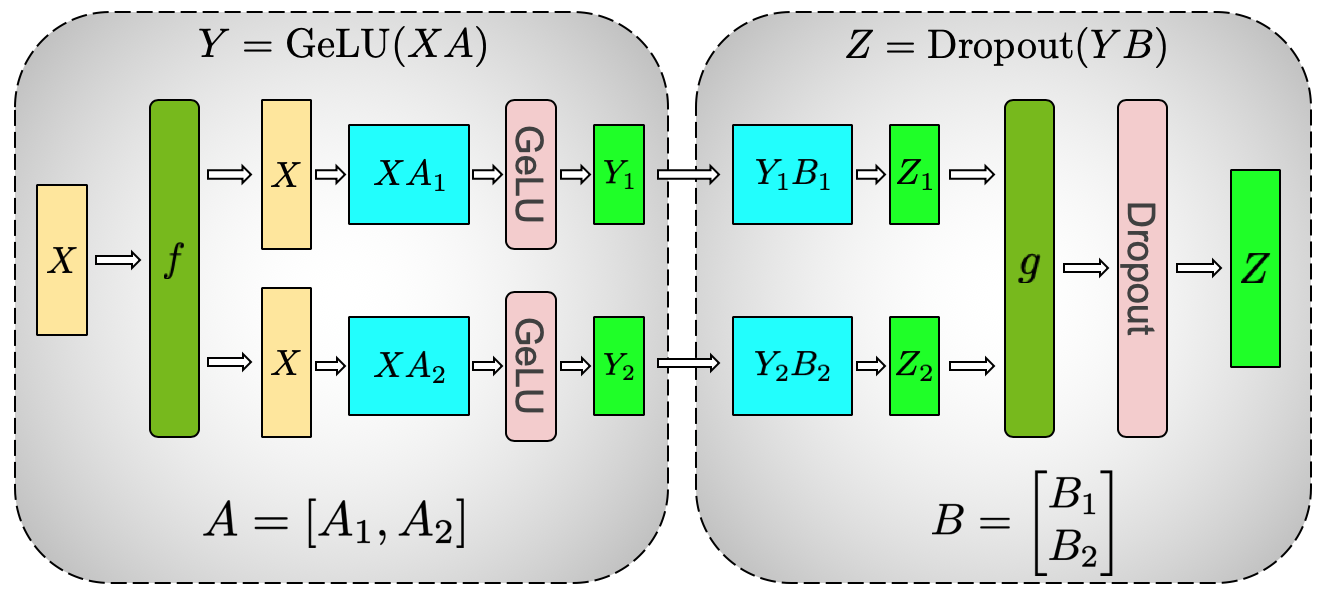
\includegraphics[scale=.33]{figures/mlp_mp_2.png}
 \caption{Tensor parallelism for the \pyinline{MLP} layers. Graphic from
 \cite{shoeybi2020megatronlm}. The $ f/g $ operations are the collective
identity/\pyinline{AllReduce} operations in the forwards pass and the \pyinline{AllReduce}/identity
operations in the backwards pass.}
 \label{fig_mlp_tensor_parallel}
\end{figure}


 \paragraph{Attention} The computations for each the $ A $ individual attention heads, which result
 in the various re-weighted values $ t ^{ a }_{ bsf } $ \eqref{eq_reweighted_values}, can be
 partitioned arbitrarily across workers without incurring any collective communications costs.  Each
 worker then holds some subset of these $ a \in \left \{ 0, \ldots , H-1 \right \} $ activations and
 the final output matrix multiply can be schematically broken up as in \begin{align} &{\rm Concat}
     \left ( \left [ t ^{ 0 }, \ldots , t ^{ H-1 } \right ] \right ) \cdot O \nn &= {\rm Concat}
     \left ( \left [ {\rm Concat}\left ( \left [ t ^{ 0 }, \ldots , t ^{ \frac{ A }{ T }-1 } \right
     ] \right ) \cdot O ^{ (0) }, \ldots ,{\rm Concat}\left ( \left [ t ^{ H-\frac{ A }{ T } },
\ldots , t ^{ A} \right ] \right ) \cdot O ^{ (T-1) } \right ] \right ) \ , \end{align} where matrix
products and concatenation both occur along the hidden dimension. That is, each worker in a group
has $ A/T $ different \pyinline{(B, S, D/A)}-shaped activations $ t ^{ a } $, which can be
concatenated into a \pyinline{(B, S, D/T)}-shaped tensor and multiplied into the
\pyinline{(D/T, D)}-shaped shard of $ O $ whose dimensions correspond to those in the just-concatenated tensor.
Concatenating together each such result from every worker (via an \pyinline{AllReduce}) gives the
desired output. The backwards pass requires similar collective communications to the \pyinline{MLP}
case above.


 \begin{figure}[ht]
     \centering
     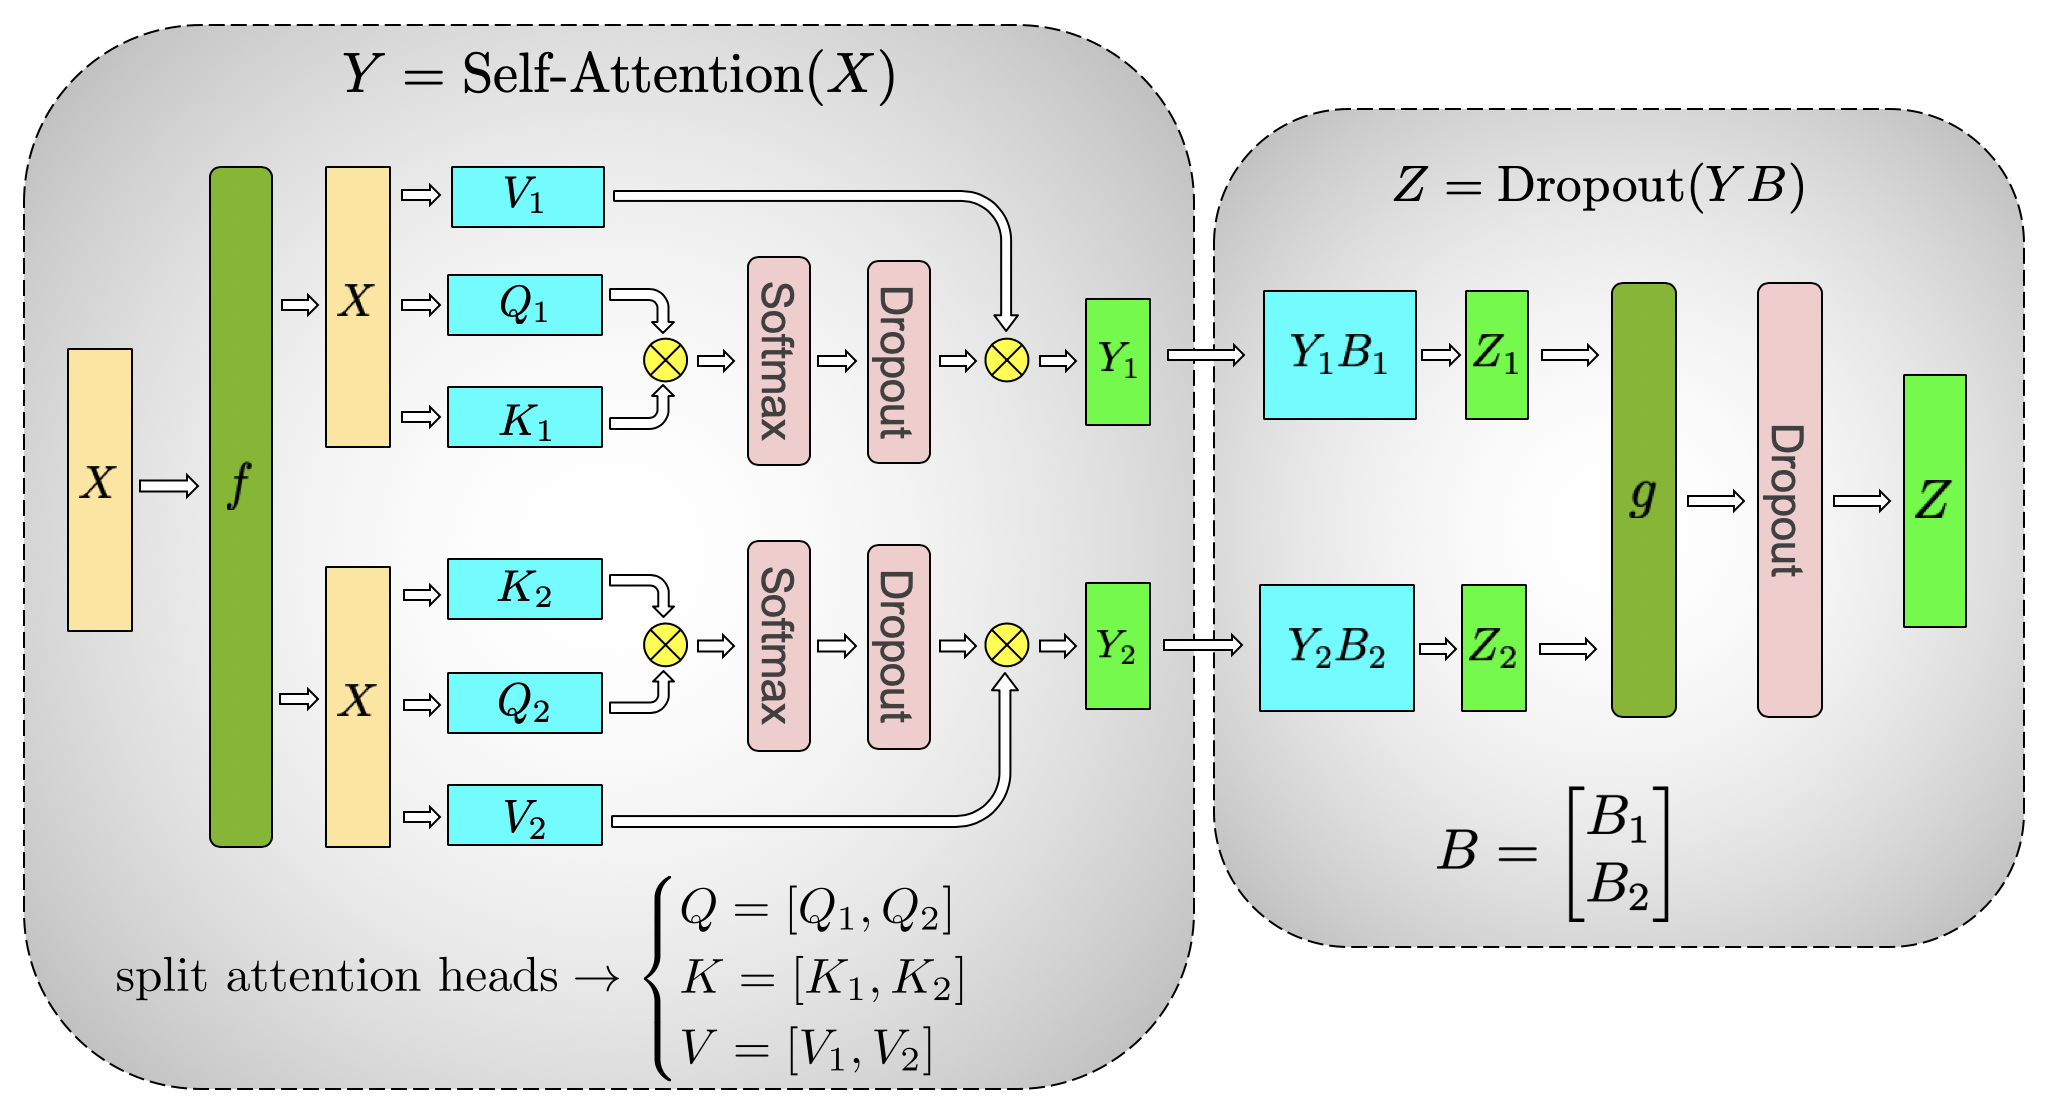
\includegraphics[scale=.45]{figures/attention_mp_2.png}
     \caption{Tensor parallelism for the \pyinline{CausalAttention} layers. Graphic from
     \cite{shoeybi2020megatronlm}. The $ f/g $ operators play the same role as in
 Fig.~\ref{fig_mlp_tensor_parallel}.}
     \label{fig_attn_tensor_parallel}
 \end{figure}

 \paragraph{Embedding and LM Head} Last, we can apply tensor parallelism to the language model head,
 which will also necessitate sharding the embedding layer, if the two share weights, as typical.

For the LM head, we shard the output dimension as should be now familiar, ending up with $ T $
different \pyinline{(B, S, V/T)}-shaped tensors, one per group member. Rather than communicating
these large tensors around and then computing the cross-entropy loss, it is more efficient to have
each worker compute their own loss where possible and then communicate the scalar losses
around\footnote{In more detail, given the gold-answers $ y _{ bs } $ for the next-token-targets, a
given worker can compute their contribution to the loss whenever their \pyinline{(B, S, V/T)}-shaped
output $ z _{ bsv' } $ contains the vocabulary dimension $ v _{ * } $ specified by $ y _{ bs } $,
otherwise those tensor components are ignored.}.

For a weight-tied embedding layer, the former construction requires \pyinline{AllReduce} in order
for every worker to get the full continuous representation of the input.

\paragraph{LayerNorm and Dropout} \pyinline{LayerNorm} instances are not sharded in pure tensor
parallelism both because there is less gain in sharding them parameter-wise, but also sharding
\pyinline{LayerNorm} in particular would require additional cross-worker communication, which we
wish to reduce as much as possible. \pyinline{Dropout} layers are also not sharded in  where
possible in pure tensor parallelism, but sharding the post-attention \pyinline{Dropout} layer is
unavoidable. It is the goal of sequence parallelism is to shard these layers efficiently; see
Sec.~\ref{subsec_seq_parallelism}.



 \paragraph{Effects on Memory} The per-worker memory savings come from the sharding of the weights
 and the reduced activation memory from sharded intermediate representations.

 The gradient and optimizer state memory cost is proportional to the number of parameters local to
 each worker (later we will also consider sharding these components to reduce redundantly-held
 information). The number of parameters per worker is reduced to
\begin{align}
    N _{ \rm params } &\approx  (4 + 2E) \frac{ L D ^{ 2 } }{ T }\ ,
    \label{eq_approx_params_tensor_parallel}
\end{align}
counting only the dominant contribution from weights which scale with $ L $, since every weight is
sharded. Since all non-activation contributions to training memory scale with $ N _{ {\rm params}  }
$, this is a pure $ 1/T $ improvement.

 The per-layer activation memory costs \eqref{eq_att_actmem_vanilla} and
 \eqref{eq_mlp_actmem_vanilla} are altered to:
\begin{align}
M _{ \rm act  } ^\texttt{Attention} &= BS \left ( \left (p + \frac{ 4p }{ T }+1 \right )D + \left
(\frac{ 2p+1 }{ T } \right )AS  \right ) \nn
M _{ \rm act  } ^\texttt{MLP} &= \left (\frac{ 2Ep }{ T }+p+1 \right )BDS\ .
\label{eq_act_mem_attn_mlp}
\end{align}
The derivation is similar to before. Adding in the (unchanged) contributions from
\pyinline{LayerNorm} instances, the total, leading order activation memory sums to
\begin{align}
    M _{ {\rm act}  } ^{ {\rm  total}  } & \approx  2BDLS   \left ( p \left (2+ \frac{ E+2 }{ T }\right ) + 1   \right )
    + ABLS ^{ 2 } \left ( \frac{ 2p+1 }{ T }\right ) \label{eq_act_mem_total_tensor_parallel}\ .
\end{align}
Again, the terms which did not receive the $ 1/T $ enhancement correspond to activations from
unsharded \pyinline{LayerNorm} and \pyinline{Dropout} instances and the $ 1/T $'s improvements can
be enacted by layering sequence parallelism on top (Sec.~\ref{subsec_seq_parallelism}).


\subsection{Sequence Parallelism \label{subsec_seq_parallelism}}

In \eqref{eq_act_mem_total_tensor_parallel}, not every factor is reduced by $ T $.
\textbf{Sequence Parallelism} fixes that by noting that the remaining contributions, which
essentially come from \pyinline{Dropout} and \pyinline{LayerNorm}, can be parallelized in the sequence dimension (as can
the residual connections).

The collective communications change a bit. If we shard the tensors across the sequence dimension
before the first \pyinline{LayerNorm}, then we want the following:
\begin{enumerate}
\item The sequence dimension must be restored for the \pyinline{CausalAttention} layer
\item The sequence should be re-split along the sequence dimension for the next \pyinline{LayerNorm} instance
\item The sequence dimension should be restored for the \pyinline{MLP} layer \footnote{This doesn't
    seem like a hard-requirement, but it's what is done in \cite{korthikanti2022reducing}.}
\end{enumerate}

The easiest way to achieve the above is the following.
\begin{enumerate}
    \item If the tensor parallelization degree is $ T $, we also use sequence parallelization degree $ T
        $.
    \item The outputs of the first \pyinline{LayerNorm} are \pyinline{AllGather}-ed to form the full-dimension
        inputs to the \pyinline{CausalAttention}  layer
    \item The tensor-parallel \pyinline{CausalAttention} layer functions much like in
        Fig.~\ref{fig_attn_tensor_parallel} \textit{except} that we do not re-form the outputs to
        full-dimensionality.  Instead, before the \pyinline{Dropout} layer, we \pyinline{ReduceScatter} them
        from being hidden-sharded to sequence-sharded and pass them through the subsequent
        \pyinline{Dropout}/\pyinline{LayerNorm} combination, similar to the first step
    \item The now-sequence-sharded tensors are reformed with another \pyinline{AllGather} to be the full-dimensionality inputs to the
        \pyinline{MLP} layer whose final outputs are similarly \pyinline{ReduceScatter}-ed to be
        sequence-sharded and are recombined with the residual stream
\end{enumerate}
The above allows the \pyinline{Dropout} mask and \pyinline{LayerNorm} weights to be sharded $ T
$-ways, but if we save the full inputs to the \pyinline{CausalAttention} and \pyinline{MLP}  layers
for the backwards pass, their contributions to the activation memory are not reduced (the $ p
$-dependent terms in \eqref{eq_act_mem_attn_mlp}). In \cite{korthikanti2022reducing}, they solve
this by only saving a $ 1/T $ shard of these inputs on each device during the forward pass and then
performing an extra \pyinline{AllGather} when needed during the backwards pass. Schematics can be
sen in Fig.~\ref{fig_tensor_seq_parallel} and Fig.~\ref{fig_tensor_seq_parallel_detail} below.

\begin{figure}[ht]
 \centering
 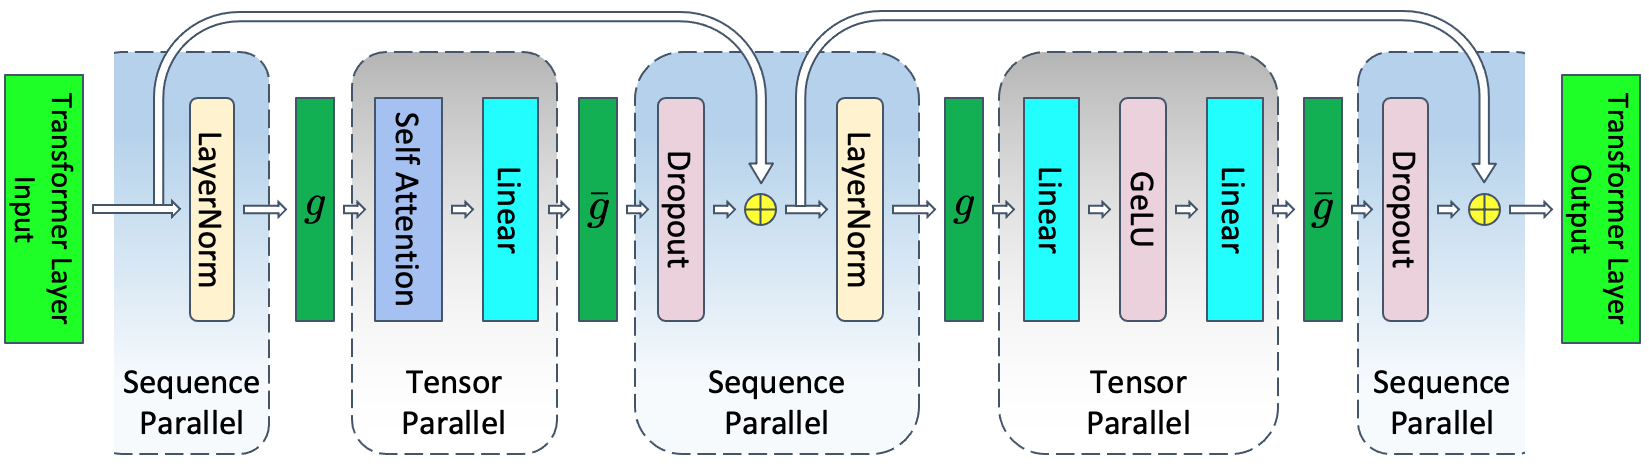
\includegraphics[scale=.25]{figures/transformer-tensor-sequence-parallel.jpg}
 \caption{Interleaved sequence and tensor parallel sections. Graphic from
 \cite{shoeybi2020megatronlm}. }
 \label{fig_tensor_seq_parallel}
\end{figure}

\begin{figure}[ht]
 \centering
 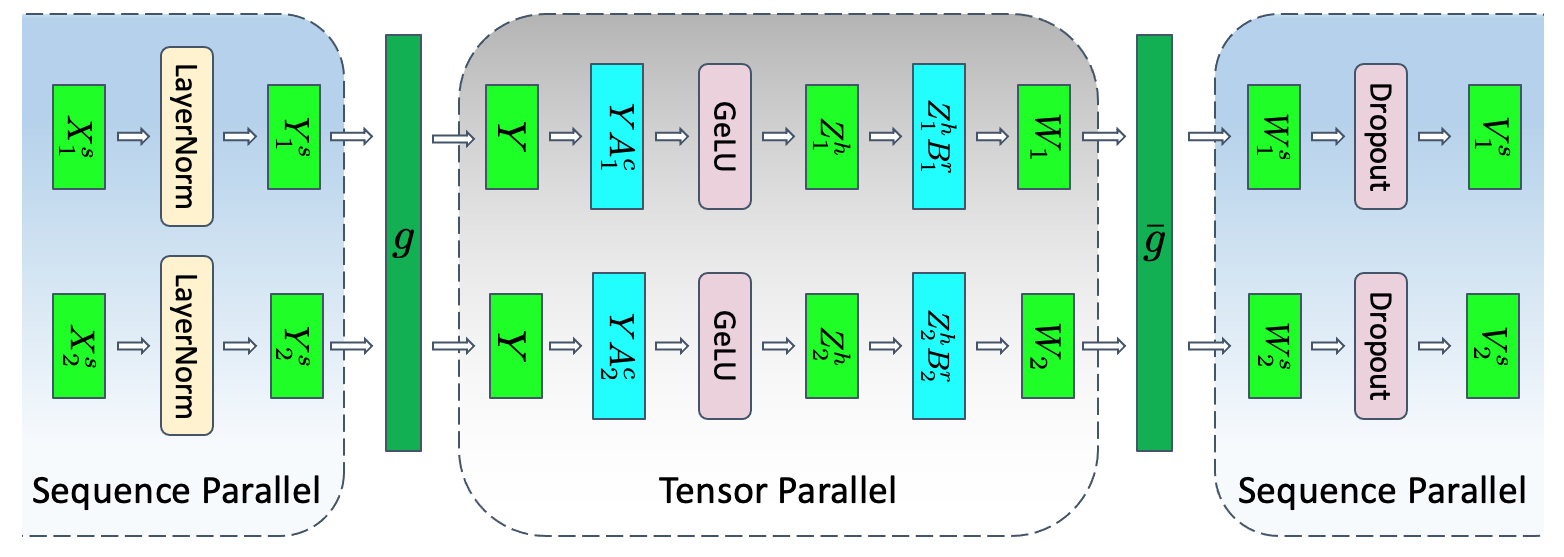
\includegraphics[scale=.25]{figures/mlp-tensor-sequence-parallel.jpg}
 \caption{Detail of the sequence-tensor parallel transition for the \pyinline{MLP} . Graphic from
 \cite{shoeybi2020megatronlm}. }
 \label{fig_tensor_seq_parallel_detail}
\end{figure}


\subsection{Pipeline Parallelism \label{subsec_pipe_parallelism}}

TODO






\subsection{Latency \label{sec_latency_train} }

\subsection{Case Study: Mixed-Precision GPT3 \label{subsec_gpt_mem_study} }

Let's run through the numbers for mixed-precision GPT3 with
\href{https://bmk.sh/2020/05/29/GPT-3-A-Brief-Summary/}{parameters}:
\begin{align}
L &= 96 \ , \quad
D = 12288 \ ,\quad
A = 96\ , \quad V = 50257\ .
 \label{eq_gpt_num}
\end{align}
We are leaving the sequence-length unspecified, but the block-size (maximum sequence-length) is $
K=2048 $.


Start by assuming no parallelism at all. The total (not per-layer!) non-activation memory is
\begin{align}
  M _{ {\rm non-act}  } ^ \texttt{GPT-3} & \approx 1463\ {\rm TiB}
\end{align}
which can be broken down further as
\begin{align}
  M _{ {\rm params}  } ^ \texttt{GPT-3} & \approx 162\ {\rm TiB} \ , \quad
 M _{ {\rm grads}  } ^ \texttt{GPT-3}  \approx 325\ {\rm TiB}\ , \quad
  M _{ {\rm optim}  } ^ \texttt{GPT-3}  \approx 975\ {\rm TiB}\ .
\end{align}
The embedding matrix only makes up $ \approx .3\% $ of the total number of parameters, justifying our
neglect of its contribution in preceding expressions.


The activation memory is
\begin{align}
  M _{ {\rm act}  } ^ \texttt{GPT-3} & \approx 3 \times 10 ^{ -2 }BS\times  \left (  1  + \frac{ S
  }{ 10 ^{ 3 } } \right ) \ {\rm TiB} \ .
\end{align}
Note that the attention matrices, which are responsible for $ \Ocal \left( S ^{ 2 } \right)  $ term, will
provide the dominant contribution to activation memory in the usual $ S \gtrsim 10 ^{ 3 } $ regime.

In the limit where we process the max block size ($ S=K=2048 $), the ratio of activation to
non-activation memory is
\begin{align}
  \frac{  M _{ {\rm act}  } ^ \texttt{GPT-3}}{ M _{ {\rm non-act}  } ^ \texttt{GPT-3} }\Big| _{
  S=2048 } & \approx  .2 B \ .
\end{align}
So, the activation memory is very significant for such models.


Using tensor parallelism into the above with the maximal $ T=8 $ which can be practically used, the
savings are significant. The total memory is now
\begin{align}
  M _{ {\rm total}  } ^{ \texttt{GPT-3}  } & \approx 187\ {\rm TiB} + 10 ^{ -2 }BS + 5 \times 10 ^{
  -6} BS ^{ 2 }\ .
\end{align}




\section{Training FLOPs \label{sec_flops_training} }

The total number of floating point operations (FLOPs)\footnote{The notation surrounding
floating-point operations is very confusing because another quantity of interest is the number
of floating-point operations a given implementation can use \textit{per-second}. Sometimes,
people use FLOPS or FLOP/s to indicate the rate, rather than the gross-count which has the lower
case ``s", FLOPs, but there's little consistency in general. We will use FLOPs and FLOP/s.}  needed to process a given batch of
data is effectively determined by the number of matrix multiplies needed.

Recall that a dot-product of the form $ v \cdot M $  with $ v \in \mathbb{R}^{ m } $ and $ M \in
\mathbb{R} ^{ m, n }$ requires $ \left (2 m-1 \right )\times n \approx 2mn$ FLOPs .
For large language models, $ m,n \sim \Ocal \left( 10 ^{ 3 } \right)  $, meaning that even expensive
element-wise operations like \pyinline{GeLU} acting on the same vector $ v $ pale in comparison by
FLOPs count \footnote{Since their FLOPs counts only scales as $ \sim \Ocal \left( n\right )  $ where
the omitted constant may be relatively large, but still negligible when all dimensions are big.}. It
is then a straightforward exercise in counting to estimate the FLOPs for a given architecture. The
input tensor is of shape \pyinline{(B, S, D)} throughout.

\begin{nicebox}{Essentials}
    The number of FLOPs to push a batch of $ B $ of sequence-length $ S $ examples through the forwards-pass
    of a decoder-only transformer is approximately $ 2BS N _{ {\rm params}  } $ where the number of
    parameters accounts for any reductions due to tensor- and sequence-parallelism\footnote{A quick argument: a
computation of the form $T _{ a _{ 0 }\ldots  a _{ n }j } =V _{ a _{ 0 }\ldots a _{ A
}i }M _{ ij } $ requires $ 2A _{ 0 }\ldots A _{ n }IJ $ FLOPs where the capital letters
represent the size of their similarly-index dimensions. Thus, the FLOPs
essentially count the size of the matrix $ M $ (that is, $ IJ $), up to a factor of 2 times all of the
dimensions in $ V $ which weren't summed over. Therefore, passing a
\pyinline{(B, S, D)}-shaped tensor through the Transformer architecture would give $ \sim 2BS\times
$(sum of sizes of all weight-matrices) FLOPs, and that this last factor is also approximately the number of
parameters in the model (since that count is dominated by weights). Thus, FLOPs $ \approx 2BSN _{
{\rm params}  } $. This is the correct as long as the self-attention FLOPs with $ \Ocal \left( S ^{ 2 } \right)$-dependence which we
didn't account for here are actually negligible (true for $ S \lesssim D $.}. The backwards-pass
    costs about twice as much as the forwards-pass. This is true as long as $ S \lesssim D $).
\end{nicebox}



\subsection{No Recomputation}

Start with the case where there is no recomputation activations.  These are the \textbf{model FLOPs} of
\cite{korthikanti2022reducing}, as compared to the \textbf{hardware FLOPs} which account for gradient
checkpointing.


\paragraph{\pyinline{CausalAttention}: Forwards }

The FLOPs costs:
\begin{itemize}
    \item  Generating the query, key, and value vectors: $ 6BSD ^{ 2 } $
    \item Attention scores:  $2BDS ^{ 2 }$
    \item Re-weighting values:  $2BDS ^{ 2 }$
    \item Final projection: $ 2BSD ^{ 2 } $
\end{itemize}

\paragraph{\pyinline{MLP}: Forwards}
Passing a  through the \pyinline{MLP} layer, the FLOPs due to the
first and second matrix-multiplies are equal, with total matrix-multiply requires $ 4BSED ^{ 2 } $.

\paragraph{Backwards Pass: Approximate}


The usual rule of thumb is to estimate the backwards pass as costing twice the flops as the forwards
pass. This estimate comes from just counting the number of $ \Ocal \left( n ^{ 2 } \right)$
matrix-multiply-like operations and seeing that for every one matrix multiplication that was needed
in the forward pass, we have roughly twice as many similar operations in the backwards pass.


The argument: consider a typical sub-computation in a neural network which is of the form $ z' =
\phi \left ( W \cdot z \right ) $ where $ z', a $ are intermediate representations $ z, z' $, $ \phi
$ is some non-linearity, and where the matrix multiply inside the activation function dominates the
forwards-pass FLOPs count, as above.  Then, in the backwards pass for this sub-computation, imagine
we are handed the upstream derivative $ \partial _{ z '  } \Lcal $. In order to complete
backpropagation, we need both to compute $ \partial  _{ W }\Lcal  $ to update $ W $ and also $
\partial  _{ z } \Lcal  $ to continue backpropagation to the next layer down. Each of these operations
 will cost about as many FLOPs as the forwards-pass, hence the estimated factor of two (but, as
 we will see, this is a very rough estimate).

 Being more precise, let $ z $ be \pyinline{(D0, ... , Dn, I)}-shaped and let $ W $ be
 \pyinline{(I, J)}-shaped such that it acts on the last index of $ z $, making $ z' $
\pyinline{(D0, ... , Dn, J)}-shaped. Denoting $D=\prod _{ i } D _{ i } $ be the number of elements
along the $ D _{ i } $ directions for brevity, the forward-FLOPs cost of the sub-computation is
therefore $ 2DIJ$.


Adding indices, the two derivatives we need are
\begin{align}
    \frac{ \partial \Lcal  }{ \partial W _{ ij } }&= \frac{ \partial \Lcal  }{ \partial z '_{ d _{ 0 } \ldots  d _{ n }j } }\phi' \left (\left (  W \cdot z \right ) _{  d _{ 0 }\ldots d _{ n }i } \right )
z _{ d _{ 0 }\ldots  d _{ n } i } \nn
   \frac{  \partial \Lcal  }{\partial  z _{ d _{ 0 }\ldots d _{ n }i } } &= \frac{ \partial \Lcal
   }{ \partial z '_{ d _{ 0 } \ldots  d _{ n }j } }\phi' \left (\left (  W \cdot z \right ) _{  d _{
   0 }\ldots d _{ n }i } \right ) W _{ ij }\ ,
\end{align}
which have shapes \pyinline{(I, J)} and \pyinline{(D0, ..., Dn, I)}, respectively. On the right
side, $ z $ and $ W \cdot  z $ are cached and the element-wise computation of $ \phi' \left ( W
\cdot z \right ) $ has negligible FLOPs count, as discussed above. The FLOPs count is instead
dominated by the broadcast-multiplies, sums, and matrix-products.

Multiplying out the first two factors which are common to each derivative involves a broadcasted
multiply of a \pyinline{(D0, ... , Dn, J)}-shaped and a \pyinline{(D0, ... , Dn, I, J)}-shaped tensor
to produce another \pyinline{(D0, ... , Dn, I, J)}-shaped result, which requires $ DIJ $ FLOPs.
The process of multiplying this factor with either $ z _{ d _{ 0 } \ldots d _{ n }i } $ or $ W _{ ij } $
and summing over the appropriate indices requires $ 2DIJ $ FLOPs for either operation, bringing the
total FLOPs to $ 5DIJ$, which is (slightly more than) double the FLOPs for this same
sub-computation in the forward-direction, hence the rough rule of thumb.


\paragraph{Backwards Pass: More Precise} \textbf{TODO}

\paragraph{Total Model FLOPs}


The grand sum is then\footnote{With a large vocabulary, the cost of the final language model head
matrix multiply can also be significant, but we have omitted its $ L $-independent,  $ 2BSDV $
contribution here. }:
\begin{align}
F _{ {\rm total}  } ^{ {\rm  model}  } &\approx 12 BDLS \left ( S + \left ( 2+E \right )D \right ) \label{eq_model_flops}\ .
\end{align}
We can also phrase the FLOPs in terms of the number of parameters \eqref{eq_approx_params_tensor_parallel} as
\begin{align}
 F _{ {\rm total}  } ^{ {\rm  model}  } \big| _{ T=1 }  &= 6BS N _{ {\rm  params}  }\times \left ( 1 + \Ocal \left( S/D\right)  \right )
\end{align}
where we took the $ T=1, D \gg S $ limit for simplicity and we note that $ BS $  is the number of
total tokens in the processed batches.

Based on the above, it is common to write down the rule of
thumb\footnote{See
\href{https://medium.com/@dzmitrybahdanau/the-flops-calculus-of-language-model-training-3b19c1f025e4}{this
blog post} or the link in Foot.~\ref{foot_eleuther_math_101}.}
\begin{align}
  \left ( {\rm Achievable \ FLOPs/sec}  \right ) \times \left ( {\rm  Training \ time}  \right )
  &\approx 6 N _{ {\rm params}  } \times \left ( {\rm Total \ tokens} \right ) \ . \label{eq_training_rule_of_thumb}
\end{align}
The above is the total compute needed to train a model with the above data.


Lastly, the \textbf{model FLOPs utilization} (MFU) is an often-quoted quantity, which is just ratio
of actually achieved FLOP/s (the rate, not the gross sum) to the maximum possible given the hardware
\begin{align}
  {\rm MFU}  &= \frac{ F _{ {\rm total}  } ^{ {\rm  model}  } \times \tau }{ \left ( {\rm Num. \ GPUs}  \right ) \times \left ( {\rm Max. \ FLOP/s/GPU}  \right ) }
\end{align}
where $ \tau $ is the throughput rate in terms of tokens/second.

\section{Scaling Laws}

\part{Inference}


\section{Basics and Problems}


The essentials of decoder-only inference is that a given input sequence $ x _{ bs } $ is turned into
a probability distribution $ p _{ bsv } $ over the vocabulary for what the next token might be.  Text
is then generated by sampling from $ p _{ bsv } $ in some way, appending that value to $ x _{ bs } $
to create a one-token-longer sequence, and then repeating until desired.

There are various problems that naive implementations of the above face:
\begin{itemize}
    \item Repeated computation from processing the same tokens in the same order repeatedly, at least for
        some sub-slice of $ x _{ bs } $.
    \item Inherently sequential computation, rather than parallel
    \item Sub-optimal sampling strategies. Just choosing the most-probably token at each new step, does
    not guarantee the most-probable overall sequence, for instance.
\end{itemize}

\section{The Bare Minimum and the kv-Cache \label{sec_kv_cache}}


There are two separate stages during generation. First, an original, to-be-continued series of prompts
$ x _{ bs }  $ can be processed in parallel to both generate the first prediction and populate any
intermediate values we may want to cache for later. We follow \cite{pope2022efficiently} and call this the
\textbf{prefill} stage. For this procedure, we require the entire $ x _{ bs } $ tensor.

In the second, iterative part of generation (the \textbf{decode} stage) we have now appended
one-or-more tokens to the sequence and we again want the next prediction, i.e. \pyinline{z[:, -1, :]}
for the last-layer outputs $ z _{ bsd } $. In this stage, we can avoid re-processing the entire $ x
_{ bs } $ tensor and get away with only processing the final, newly added token, \textit{if} we are
clever and cache old results.

The important pieces occur in the \pyinline{CausalAttention} layer, as that's the only location in
which the sequence index is not completely parallelized across operations. Referring back to
Sec.~\ref{subsubsec_attn_layer}, given the input $ z _{ bsd } $ of the \pyinline{CausalAttention}
layer, the re-weighted value vectors\footnote{Summed over $ s' $, but concatenating the different $
a $ values over the $ f $ dimension.} $ w ^{ a }_{ bss'd } v ^{ a } _{ bs'f } $ are the key objects
which determine the next-token-prediction, which only depends on the $ s=-1 $ index values.
Therefore, we can cut out many steps and minimum requirements are:
\begin{itemize}
    \item Only the attention weights $ w ^{ a }_{ bss'd }$ with $ s=-1 $ are needed
    \item The only query values $ q ^{ a }_{ bsd } $ needed to get the above are those with $ s=-1 $
    \item Every component of the key and value vectors $k ^{ a }_{ bsd }, v ^{ a }_{ bsd } $ is
        needed, but because of the causal mask, all components except for the last in the sequence
        dimension ($ s\neq -1 $) are the same as they were in the last iteration, up to a shift
        by one position\footnote{That is, if we add a label $ t $ which indexes the iteration of generation
        we are on, then $ z ^{ (t+1) } _{ bsd } = z ^{ (t)} _{ b (s-1)d } $ for every tensor in the network, except for when $ s=-1 $, the last position.}
\end{itemize}

So, we are led to the concept of the \textbf{kv-cache} in which we cache old key and query vectors for generation.
The cache represents a tradeoff: fewer FLOPs are needed for inference, but the memory costs are potentially
enormous, since the size of the cache grows with batch size and sequence length:
\begin{align}
    M _{ {\rm kv-cache}  } &= 2pBSDL /T\ ,  \label{eq_kv_cache_memory}
\end{align}
in the general case with tensor-parallelism. This can easily be larger than the memory costs of the
model parameter: $ M _{ {\rm params}  } ^{ {\rm  inference}  } \sim p N _{ {\rm params}  } \sim p LD
^{ 2 }  $ (dropping $ \Ocal \left( 1 \right)  $ factors), so that the cache takes up more memory
when $ BS \gtrsim D $. Also, re-processing an entire input sequence every time also exhibits the
usual $\sim S ^{ 2 }  $ FLOPs dependence, but this is reduced to being \textit{linear} in $ S $
when the kv-cache is used.



\section{Basic Memory, FLOPs, and Latency}

The analysis of the memory and FLOPs for inference is much simpler than its corresponding training
counterparts (Sec.~\ref{sec_flops_training} and Sec.~\ref{sec_memory_training}  ), since there is no
optimizer state and activations can be thrown away immediately after use (neglecting the kv-cache).
We cover naive inference without a kv-cache first, then repeat the analysis with the cache. Much of
this is based on \cite{kipply_inference_math}.

\paragraph{Naive Inference} Processing a single \pyinline{(B, S, D)}-shaped tensor to generate a single
next input costs the $ 2BSN _{ {\rm params}  } $ FLOPs we found for the forwards-pass in
Sec.~\ref{sec_flops_training}. Memory costs just come from the parameters themselves: $ M _{ {\rm
infer.}  }^{ {\rm naive}  }=pN _{ {\rm params}  } $. Per the analysis of App.~\ref{app_flops_mem_bound},
naive inference is compute-bound and so the per-token-latency is approximately\footnote{Assuming we
do the naive thing here and generate the next token in a similarly naive way, shifting over the
context window.}  $  2BSN _{ {\rm params}  }/ \lambda _{ {\rm FLOPs}  } $ where the FLOPs bandwidth
in the denominator is again defined in App.~\ref{app_flops_mem_bound}.

\paragraph{kv-Cache Inference}
The FLOPs requirements for the hidden-dimension matrix multiplies during generation are $2BN _{ {\rm params}  } $,
since we are only processing a single token, per previous results.   This is in addition to the up-front cost of $ 2BSN _{
{\rm params}} $ for the prefill. But, the memory requirements are raised to \begin{align} M _{ {\rm
infer.}  }^{ {\rm kv-cache}  } &=pN _{ {\rm params}  } + 2pBSDL/T\ . \end{align} The computation is
now compute bound (again, see App.~\ref{app_flops_mem_bound}) and has per-token-latency of
approximately $ M _{ {\rm infer.} }/ \lambda _{ {\rm mem.} }$, unless the batch-size is very large.



\section{Case Study: \href{https://huggingface.co/tiiuae/falcon-40b-instruct?_sm_vck=j230jZ2ssDkkPfJTfRt6tjQNTQZJ65N7VDWmj5Ff6f3jZ3mhh2Pq}{Falcon-40B}}

Let's work through the details of the kv-cache for Falcon-40B\footnote{Falcon actually uses
multi-query attention, which changes the computations here, but we will pretend it does not in this
section for simplicity.} with $ D=8192 $, $ L=60 $, $ S=2048 $.  In half, $ p=2 $ precision, the model weights just about fit on an
80GiB A100, but this leaves no room for the cache, so we parallelize $ T $ ways across $ T $ GPUs,
assumed to be on the same node. The total memory costs are then
\begin{align}
    M _{ {\rm  total} } &\approx  \frac{ {\rm 80GiB} + {\rm 4GiB}\times B }{ T } \ .
\end{align}
This means that in order to hit the compute-bound threshold of $ B \sim 200 $ (see
App.~\ref{app_flops_mem_bound}) we need at least $ T=4 $ way parallelism.  Taking $ T=4 $, and running
at capacity with $ B \sim 200$ so that we are compute-bound, the per-token-per-batch latency from computation alone
is approximately $ \frac{ pN _{ {\rm params} } }{ \lambda _{ {\rm FLOPs} } T} \sim $13ms. While the
memory-bandwidth time $ M _{ {\rm total} } / \lambda _{ {\rm mem} } $ is of a comparable size, we assume
that the computations are immediately starting as the data is streamed from memory, such that these
costs are not additive.












\appendix



\section{Conventions and Notation\label{app_conventions}}


We loosely follow the conventions of \cite{korthikanti2022reducing} and denote the main Transformers
parameters by:
\begin{itemize}
    \item $ A $: number of attention heads
    \item $ B $: microbatch size
    \item $ D $: the hidden dimension size
    \item $ E $: expansion factor for MLP layer (usually $ E=4 $)
    \item $ F $: FLOPs
    \item $ K $: the block size (maximum sequence length\footnote{In the absence of methods such as         ALiBi \cite{ALiBi}  can be used to extend the sequence length at inference time.})
    \item $ L $: number of transformer layers
    \item $ N _{ {\rm params}  } $: number of model parameters held by a given device
    \item $ P $: pipeline parallel size
    \item $ S $: input sequence length
    \item $ T $: tensor parallel size
    \item $ V $: vocabulary size
    \item $ \tau $: throughput rate in tokens/second
    \item $ p $: the precision of the elements of a tensor in bytes
    \item $ \lambda  $: used for various rates, e.g. $ \lambda _{ {\rm mem}  } $ is memory bandwidth
\end{itemize}
Where it makes sense, we try to use the lower-case versions of these characters to denote the
corresponding indices on various tensors. For instance, an input tensor with the above batch size,
sequence length, and vocabulary size would be written as $ x _{ bsv } $, with $ b \in \left \{ 0,
\ldots, B - 1 \right \} $, $ s \in \left \{ 0, \ldots, S - 1\right \} $, and $  v \in \left \{ 0,
    \ldots, V -1\right \}$ in math notation, or as \mintinline{python}{x[b, s, v]} in code.  Typical
    transformers belong to the regime
\begin{gather}
V \gg D, S \gg L, A \gg P, T \ .  \label{app_eq_transformers_approxs}
\end{gather}
For instance, GPT-2 and GPT-3 \cite{gpt2radford2019language, gpt3brown2020language} have $ V \sim \Ocal \left( 10 ^{ 4 } \right)  $,
$ S, L \sim \Ocal \left( 10 ^{ 3 } \right)  $, $ L, A \sim \Ocal \left( 10 ^{ 2 } \right)  $. We
will often assume that\footnote{This condition ensures that the $ \Ocal \left( S ^{ 2 } \right)  $
    FLOPs cost from self-attention is negligible compared to $ \Ocal \left( D ^{ 2 } \right)  $
    contributions from other matrix multiplies.  It should be noted that in Summer 2023 we are
steadily pushing into the regime where this condition does \textit{not}  hold.} $ S \lesssim D $.

As indicated above,  we use zero-indexing. We also use \pyinline{python} code
throughout\footnote{Written in a style conducive to latex, e.g. no type-hints and clarity
prioritized over optimization.}  and
write all ML code using standard \pyinline{torch} syntax. To avoid needing to come up with new
symbols in math expressions we will often use expressions like $ x \leftarrow f(x) $ to refer to performing
a computation on some argument ($ x $) and assigning the result right back to the variable $ x $
again.

Physicists often joke (half-seriously) that Einstein's greatest contribution to physics was his
summation notation in which index-sums are implied by the presence of repeated indices and summation
symbols are entirely omitted. For instance, the dot product between two vectors would be written as
\begin{align}
    \vec{x} \cdot \vec{y} &= \sum _{ i } x _{ i } y _{ i } \equiv x _{ i } y _{  i }
    \label{app_eq_einstein_sum}
\end{align}
We use similar notation which is further adapted to the common element-wise deep-learning
operations.  The general rule is that if a repeated index appears on one side of an equation, but
not the other, then a sum is implied, but if the same index appears on both sides, then it's an
element-wise operation. The Hadamard-product between two matrices $ A $ and $ B $ is just
\begin{align}
  C _{ ij } &= A _{ ij } B _{ ij }\ .
\end{align}
Einstein notation also has implementations available for \pyinline{torch}:
\href{https://rockt.github.io/2018/04/30/einsum}{see this blog post on \pyinline{einsum}} or the
\href{https://einops.rocks/1-einops-basics/}{\pyinline{einops}} package.

 We also put explicit indices on operators such as Softmax to help clarify the relevant
 dimension, e.g. we would write the softmax operation over the $ b $-index of some batched
 tensor $ x _{ bvd\ldots } $ as
 \begin{align}
     s _{ bvd\ldots } &= \frac{ e^{ x _{ bv d\ldots}  } }{ \sum _{ v = 0 } ^{  v= V-1 } e^{ x _{
     bvd\ldots } } } \equiv
     \Sm _{ v } \ x _{ bvd\ldots }
     \ , \label{app_eq_einstein_softmax}
 \end{align}
 indicating that the sum over the singled-out $ v $-index is gives unity.

\section{Collective Communications \label{app_collective_communications} }

A quick refresher on common distributed
\href{https://docs.nvidia.com/deeplearning/nccl/user-guide/docs/usage/collectives.html}{communication
primitives}.  Consider $ N $ workers with tensor data $ x ^{ (n) }  $ of some arbitrary shape
\pyinline{x.shape}, where $ n $ labels the worker and any indices on the data are suppressed. The $
n=0 $ worker is arbitrarily denoted the \textit{chief}.  Then, the primitive operations are:
\begin{itemize}
    \item \pyinline{Broadcast}: all workers receive  the chief's data, $ x ^{ (0) }  $.
    \item \pyinline{Gather}: all workers communicate their data $ x _{ n } $ to the chief, e.g. in a
        concatenated array $ [x ^{ 0 }, x ^{ 1 }, \ldots , x ^{ N-1 }] $.
    \item \pyinline{Reduce}: data is \pyinline{Gather}-ed to the chief, which then performs some
        operation (\pyinline{sum}, \pyinline{max}, \pyinline{concatenate}, etc.) producing a new tensor $
        x' $ on the chief worker.
    \item \pyinline{AllGather}: \pyinline{Gather} followed by \pyinline{Broadcast}, such that all
        data $ x ^{ (n) } $ is communicated to all workers.
    \item \pyinline{AllReduce}: generalization of \pyinline{Reduce} where all
        workers receive the same tensor $ x' $ produced by operating on the $ x ^{ (n) } $.
        Equivalent to a \pyinline{Reduce} followed by \pyinline{Broadcast}, or a
        \pyinline{ReduceScatter} followed by a \pyinline{AllGather} (the more efficient
        choice\footnote{The former strategy scales linearly with the number of worker, while the
            latter strategy underlies ``ring" \pyinline{AllReduce} which is (nearly) independent of
            the number of workers.
            \href{https://andrew.gibiansky.com/blog/machine-learning/baidu-allreduce/}{See this blog
                post for a nice visualization} or \cite{bandwidthOptimalAllReduce2009} for a
            relevant paper.\label{foot_all_reduce}}).
    \item \pyinline{ReduceScatter}: a reducing operation is applied to the $ x ^{ (n) } $ to produce
        a $ x' $ of the same shape, but each worker only receives a slice $ 1/N $ of the result.
\end{itemize}



\section{Hardware}

Basic information about relevant hardware considerations.


\subsection{NVIDIA GPU Stats \label{app_gpu_stats}}


Summary of relevant NVIDIA GPU statistics:
\begin{center}
\begin{tabular}{| c |c| c |c |c| c| }\hline
    GPU & Memory & $ \lambda _{ {\rm FLOP/s }  } $& $ \lambda _{ {\rm mem}  } $  & $ \lambda _{ {\rm math}  } $  & $ \lambda _{ {\rm comms}  } $\\ \hline
    \href{https://www.nvidia.com/content/dam/en-zz/Solutions/Data-Center/a100/pdf/nvidia-a100-datasheet.pdf}{A100}& 40GiB&  312  TFLOP/s &   1.6 TiB/s  & 195 FLOPS/B & 300 GiB/s \\ \hline
    \href{https://www.nvidia.com/content/dam/en-zz/Solutions/Data-Center/a100/pdf/nvidia-a100-datasheet-nvidia-us-2188504-web.pdf}{A100} & 80GiB&  312  TFLOP/s &   2.0 TiB/s  & 156 FLOPS/B & 300 GiB/s \\ \hline
    \href{https://images.nvidia.com/content/technologies/volta/pdf/volta-v100-datasheet-update-us-1165301-r5.pdf}{V100} & 32GiB&  130  TFLOP/s &   1.1 TiB/s  & 118  FLOPS/B & 16 GiB/s \\ \hline
\end{tabular}
\end{center}
where
\begin{itemize}
    \item $ \lambda _{ {\rm  FLOP/s}  } $ is flops bandwidth (for \pyinline{float16/bfloat16}  multiply-accumulate ops)
    \item $ \lambda _{ {\rm  mem}  } $ is memory bandwidth
    \item $ \lambda _{ {\rm  math}  } = \frac{  \lambda _{ {\rm FLOP/s}  } }{ \lambda _{ {\rm mem} } } $ is \href{https://docs.nvidia.com/deeplearning/performance/dl-performance-gpu-background/index.html#gpu-arch}{math bandwidth}
    \item $ \lambda _{ {\rm  comms}  } $ is one-way communication bandwidth
\end{itemize}




\section{Compute-bound vs Memory-bound \label{app_flops_mem_bound} }

If your matrix-multiplies are not sufficiently large on,
you are wasting resources \cite{he2022brrrrfromfirstprinciples}. The relevant parameters which
determine sufficiency are $ \lambda _{ {\rm FLOP/s}  } $ and $ \lambda _{ {\rm mem}  } $, the FLOPs
and memory bandwidth, respectively. The ratio $  \lambda _{ {\rm math}  } \equiv \frac{  \lambda _{ {\rm FLOP/s}  } }{ \lambda _{ {\rm mem}  } }   $
determines how many FLOPS you must perform for each byte loaded from memory; see App.~\ref{app_gpu_stats}.
If your computations have a FLOPs/B ratio which is larger than  $ \lambda _{ {\rm math}  } $, then
you are compute-bound (which is good, as you're maximizing compute), and otherwise you are
memory(-bandwidth)-bound (which is bad, since your compute capabilities are idling). The FLOPs/B
ratio of your computation is sometimes called the \textbf{compute intensity} or \textbf{arithmetic
intensity}. When compute bound, a process takes time $ \sim F/\lambda _{ {\rm FLOPs} } $, while
memory-bound processes take time\footnote{Note that the time is not additive, e.g. compute-bound tasks do
not take time $ \sim F/\lambda _{ {\rm FLOPs} } +M/\lambda _{ {\rm mem} }$ because they are not sequential: compute and memory-communications can be concurrent.} $ \sim M/\lambda _{ {\rm mem} } $.


For instance, to multiply a \pyinline{(B, S, D)}-shaped tensor $ z _{ bsd } $ by a \pyinline{(D, D)}-shaped
weight-matrix $ W _{ d d' } $, $ p \left ( BSD +D ^{ 2 } \right ) $ bytes must be transferred from
DRAM to SRAM at a rate $ \lambda _{ {\rm  mem}  } $, after which we perform $ 2BSD ^{ 2 } $ FLOPs,
and write the \pyinline{(B, S, D)}-shaped  result back to DRAM again, for a ratio of
\begin{align}
    \frac{ 1 }{ p } \frac{ BSD }{ 2BS + D } \ \left ( {\rm FLOPs/B} \right )  \ .
\end{align}
We want to compare this against $ \lambda _{ {\rm math}  } $, which from
App.~\ref{app_gpu_stats} we take to be $ \Ocal \left( 100\  {\rm FLOPs/B} \right)  $, and plugging
in any realistic numbers, shows that such matrix-multiplies are essentially always compute-bound.
Compare this to the case of some element-wise operation applied to the same $ z _{ bsd } $ tensor
whose FLOPs requirements are $ \sim C\times BSD $ for some constant-factor $ C \ll S, D $.  Then,
then FLOPS-to-bytes ratio is $ \sim \frac{ C }{ p } $, which is \textit{always} memory-bound for
realistic values of $ C $. The moral is to try and maximize the number of matrix-multiplies and
remove as many element-wise operations that you can get away with.


Finally, we note that the above has implications for the Transformers architecture as a whole, and
in particular it highlights the difficulties in efficient inference. Under the assumptions of
Sec.~\ref{sec_flops_training}, $ \sim \Ocal \left( BSN _{ {\rm params}  }  \right)  $
total FLOPs needed during training, while the number of bytes loaded from and written to memory are
$ \Ocal \left( BSDL + N _{ {\rm params}  } \right)  \sim \Ocal \left( \frac{ BS N _{ {\rm params}  } }{ D}+ N _{ {\rm params}  } \right)  $
which is $ \Ocal \left( N _{ {\rm  parama}  } \right)  $ for not-super-long sequence lengths.  The
arithmetic intensity is therefore $ \Ocal \left( BS \right)  $ and so training is compute-bound in any
usual scenario, as long as individual operations in the network don't suffer from outlandish
memory-boundedness. The problem during inference is that (if using the kv-cache; see
Sec.~\ref{sec_kv_cache}) we only need to process a \textit{single} token at a time and so $ S
\longrightarrow 1 $ in the preceding and the arithmetic intensity drops to $ \Ocal \left( B \right)
$. On our favorite 80GiB A100s, we then need to be able to process batch sizes $ B \sim \Ocal \left(
200 \right)  $ in order to saturate our compute. This is hard, which is why efficient inference is
hard \cite{kipply_inference_math} .

 \section{TODO}


 \begin{itemize}
 \item Tokenizers
 \item Generation
 \item Activations
 \item Flash attention
 \item BERT family
 \item Residual stream
 \item Scaling laws
 \item Cheat sheet
 \end{itemize}

\bibliographystyle{latex_goon/utphys}
\bibliography{bibliography}
\end{document}




